\chapter{Workloads}
\label{sec:workloads}

%%%%%%%%%%%%%%%%%%%%%%%%%%%%%%%%%%%%%%%%%%%%%%%%%%%%%%%%%%%%%%%%%%%%%%%%%%%%%%
%%%%%%%%%%%%%%%%%%%%%%%%%%%%%%%%%%%%%%%%%%%%%%%%%%%%%%%%%%%%%%%%%%%%%%%%%%%%%%
%%%%%%%%%%%%%%%%%%%%%%%%%%%%%%%%%%%%%%%%%%%%%%%%%%%%%%%%%%%%%%%%%%%%%%%%%%%%%%

\section{Query Description Format}
\label{sub:queries_structure}
Queries are described in natural language using a well-defined structure that consists of three sections:
\textit{description}, a concise textual description of the query;
\textit{parameters}, a list of input parameters and their types;
and \textit{results}, a list of expected results and their types.
We use the following notation:

\begin{itemize}
    \item \textbf{Entity}: entity type in the dataset.\\
        One word, possibly constructed by appending multiple words together, starting with uppercase character and following the camel case notation,
        \eg \textsf{TagClass} represents an entity of type ``TagClass''.
    \item \textbf{Relationship}: relationship type in the dataset.\\
        One word, possibly constructed by appending multiple words together, starting with lowercase character and following the camel case notation,
        and surrounded by arrow to communicate direction,
        \eg \mbox{\textsf{-workAt->}} represents a directed relationship of type ``workAt''.
    \item \textbf{Attribute}: attribute of an entity or relationship in the dataset.\\
        One word, possibly constructed by appending multiple words together, starting with lowercase character and following the camel case notation,
        and prefixed by a ``.'' to dereference the entity/relationship,
        \eg \textsf{Person.firstName} refers to ``firstName'' attribute on the ``Person'' entity,
        and \mbox{\textsf{-studyAt->.classYear}} refers to ``classYear'' attribute on the ``studyAt'' relationship.
    \item \textbf{Unordered Set}: an unordered collection of distinct elements.\\
        Surrounded by \{ and \} braces, with the element type between them,
        \eg \textsf{\{String\}} refers to a set of strings.
    \item \textbf{Ordered List}: an ordered collection where duplicate elements are allowed.\\
        Surrounded by [ and ] braces, with the element type between them,
        \eg \textsf{[String]} refers to a list of strings.
    \item \textbf{Ordered Tuple}: a fixed-length, fixed-order list of elements, where elements at each position of the tuple have predefined, possibly different, types. \\
        Surrounded by < and > braces, with the element types between them in a specific order
        \eg \textsf{<String, Boolean>} refers to a 2-tuple containing a string value in the first element and a boolean value in the second,
        and \textsf{\{<String, Boolean>\}} is an ordered list of those 2-tuples.
\end{itemize}

\paragraph{Categorization of results.} Results are categorized according to their source of origin:

\begin{itemize}
	\item \textbf{Raw} (\texttt{R}), if the result attribute is returned with an unmodified value and type.
	\item \textbf{Calculated} (\texttt{C}), if the result is calculated from attributes using arithmetic operators, functions, boolean conditions, etc.
	\item \textbf{Aggregated} (\texttt{A}), if the result is an aggregated value, \eg a count or a sum of another value. If a result is both calculated and aggregated (\eg $\mathsf{count(x) + count(y)}$ or $\mathsf{avg(x + y)}$), it is considered an aggregated result.
	\item \textbf{Meta} (\texttt{M}), if the result is based on type information, \eg the type of a node.
\end{itemize}


%%%%%%%%%%%%%%%%%%%%%%%%%%%%%%%%%%%%%%%%%%%%%%%%%%%%%%%%%%%%%%%%%%%%%%%%%%%%%%
%%%%%%%%%%%%%%%%%%%%%%%%%%%%%%%%%%%%%%%%%%%%%%%%%%%%%%%%%%%%%%%%%%%%%%%%%%%%%%
%%%%%%%%%%%%%%%%%%%%%%%%%%%%%%%%%%%%%%%%%%%%%%%%%%%%%%%%%%%%%%%%%%%%%%%%%%%%%%

\section{Conventions for Query Definitions}

\paragraph{Interval notations.} Closed interval boundaries are denoted with 
\texttt{[} 
and \texttt{]}, while open interval boundaries are denoted with \texttt{(} and 
\texttt{)}. For example, \texttt{[0, 1)} denotes an interval between 0 and 1, 
closed on the left and open on the right.

\paragraph{Comparing Date and DateTime values.}

Some query specifications (\eg \queryRefCard{bi-read-01}{BI}{1}) require implementations to compare a
$\mathsf{DateTime}$ value with a $\mathsf{Date}$ value. In these cases, the 
$\mathsf{Date}$ value should be implicitly converted $\mathsf{DateTime}$ value 
with a time of 00:00:00.000+0000 (\ie with the timezone of GMT).

\paragraph{Matching semantics.}

Unless noted otherwise, the specification uses \emph{homomorphic} matching 
semantics~\cite{DBLP:journals/csur/AnglesABHRV17}, \ie both nodes and edges can 
occur multiple times in a match. Note that for variable-length path, duplicate 
edges are not allowed.

\paragraph{Aggregation semantics.}

The \lstinline{count} aggregation always requires the query to determine the number of \emph{distinct} elements (nodes or edges). For example, this can be achieved in the Cypher, SPARQL and SQL query languages with the \lstinline[language=sql]{count(DISTINCT ...)} construct.

\paragraph{Graph patterns.}

To illustrate queries, we use graph patterns such as \autoref{fig:example-graph-pattern} with the following notation:

\begin{figure}[ht]
	\begin{center}
		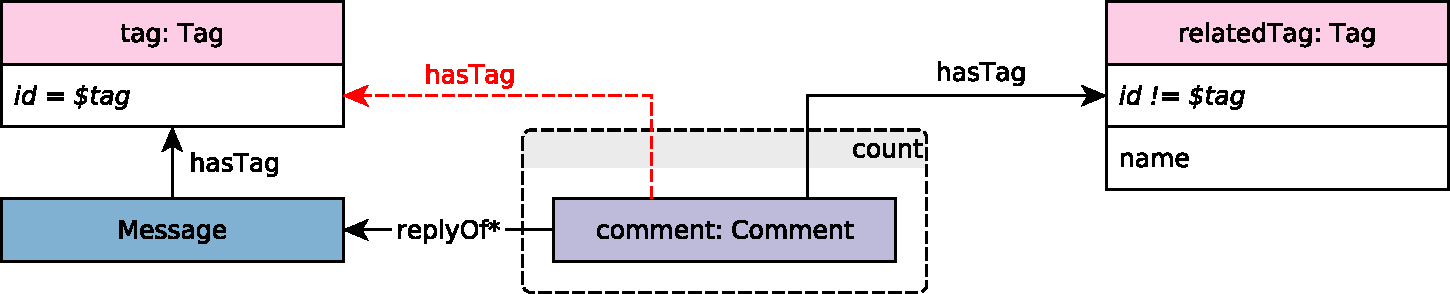
\includegraphics[scale=\patternscale,margin=0cm .2cm]{patterns/bi-read-08}
		\caption{Example graph pattern.}
		\label{fig:example-graph-pattern}
	\end{center}
\end{figure}

\begin{itemize}
	\item Nodes in the pattern are shown with rectangular boxes with their type name stated at the top and emphasized with colour coding.
	Thick solid borders denote that the node is uniquely specified by the query parameters (\eg by using an identifier or a unique attribute such as $\mathsf{name}$ and $\mathsf{URL}$ for certain types). Thick dashed borders denote that the query parameters filter for instances of the type (\eg ones created in a certain time period).
	\item Nodes in the pattern are captioned with $\mathsf{entityName: EntityType}$ (camel case 
	notation for both, starting with a lowercase character for the first and an 
	uppercase character for the second). If the $\mathsf{entityName}$ is neither returned in the query results (in raw, aggregated, or calculated form), nor referenced in the query specification, the $\mathsf{entityName}$ can be omitted.
	\item Regular edges in the pattern, \ie edges that must be present in the subgraph, are denoted with solid lines.
	\item Negative edges, \ie edges that must not be present in the subgraph, are denoted with \textcolor{red}{\dashuline{dashed red}} lines and the \guillemotleft neg\guillemotright\ keyword.
	\item Optional edges, \ie edges that may or may not be in the subgraph, are denoted with \dashuline{dashed} lines and the \guillemotleft opt\guillemotright\ keyword.
	\item Edges without direction imply that there must be an edge in \emph{the least one of the (incoming, outgoing) directions}.
	\item Filtering conditions are typeset in \textit{italic}, \eg $\textit{id = 
	\textdollar tag}$.
	\item Attributes that should be returned are denoted in sans-serif font, \eg $\mathsf{name}$.
	\item Variable length paths, \ie edges that can be traversed multiple times 
	are denoted with $*\mathsf{min}...\mathsf{max}$, \eg $\mathsf{replyOf}*$ or 
	$\mathsf{knows*1 \ldots 2}$. By default, the value of $\mathsf{min}$ is 1, 
	and the value of $\mathsf{max}$ is unlimited.
	\item Aggregations are shown in boxes with a grey strip on their top describing the type of aggregation ($\mathsf{count}$, $\mathsf{sum}$, $\mathsf{avg}$, etc.).
\end{itemize}

\newcommand{\tuple}[1]{\langle #1 \rangle}

\paragraph{Keywords.} The pattern notation uses a small set of keywords:

\begin{itemize}
	\item Aggregation operations: \lstinline{count}, \lstinline{avg}, \lstinline{sum}
	\item Functions:
	\begin{itemize}
		\item \lstinline{floor(x)}: returns $\lfloor x \rfloor$,
		\item \lstinline{year(date)}: extracts the year from a given date,
		\item \lstinline{month(date)}: extracts the month from a given date.
		\item \lstinline{day(date)}: extracts the day (of the month) from a given date.
	\end{itemize}
\end{itemize}

\paragraph{Resolving ambiguity.} Note that if the textual description and the graph pattern are different for a particular query (either due to an error or the lack of sophistication in the graphical syntax), \emph{the textual description takes precedence}.

%%%%%%%%%%%%%%%%%%%%%%%%%%%%%%%%%%%%%%%%%%%%%%%%%%%%%%%%%%%%%%%%%%%%%%%%%%%%%%
%%%%%%%%%%%%%%%%%%%%%%%%%%%%%%%%%%%%%%%%%%%%%%%%%%%%%%%%%%%%%%%%%%%%%%%%%%%%%%
%%%%%%%%%%%%%%%%%%%%%%%%%%%%%%%%%%%%%%%%%%%%%%%%%%%%%%%%%%%%%%%%%%%%%%%%%%%%%%

\section{Substitution Parameters}

\input{substitution-parameters}

%%%%%%%%%%%%%%%%%%%%%%%%%%%%%%%%%%%%%%%%%%%%%%%%%%%%%%%%%%%%%%%%%%%%%%%%%%%%%%
%%%%%%%%%%%%%%%%%%%%%%%%%%%%%%%%%%%%%%%%%%%%%%%%%%%%%%%%%%%%%%%%%%%%%%%%%%%%%%
%%%%%%%%%%%%%%%%%%%%%%%%%%%%%%%%%%%%%%%%%%%%%%%%%%%%%%%%%%%%%%%%%%%%%%%%%%%%%%

\section{Load Definition}

\input{load-definition}
